\documentclass{article}
\usepackage{graphicx}
\usepackage[T1]{fontenc}

\begin{document}
	
	\title{Week 1}
	\author{Nico Limacher}
	
\maketitle

\section{Introduction}

	\subsection*{\centerline{What is Machine Learning}}
	
		No well accepted definition, but here's Arthur Samuel back in the day:
		\begin{quote}
			The field of study that gives computers the ability to learn without being explicitly learned.
		\end{quote}
		More recently defined by Tom Mitchell of Carnegie Mellon: 
		\begin{quote}
			A computer program is said to learn from experience E with respect to some task T and some performance measure P, if its performance on T, as measured by P, improves with experience E.
		\end{quote}
		In the case of an email spam filter:
		\begin{description}
			\item[T:] Classifying emails as spam
			\item[P:] The proportion of emails correctly marked as spam
			\item[E:] Observing the user mark certain emails themselves
		\end{description}
		Some goals:
		\begin{itemize}
			\itemsep0em
			\item Discuss Supervised Learning
			\item Discuss Unsupervised Learning
			\item Get practical advice for implementation of such methods
		\end{itemize}
		
	\subsection*{\centerline{Supervised Learning}}
	
		\paragraph*{Formal Definition} The task of learning a function that maps an input to an output based on example input-output pairs. It infers a function from labeled training data consisting of a set of training examples.
		\\\\Essentially, for every example data point in our set we are told the correct answer.
		
		\subsubsection*{Example 1: Housing Data in Portland, Oregon}
		Given data in Figure 1. if you own a house with 750 sq. ft., how much can you expect the house to be worth?
		\begin{figure}[h!]
			\centering
			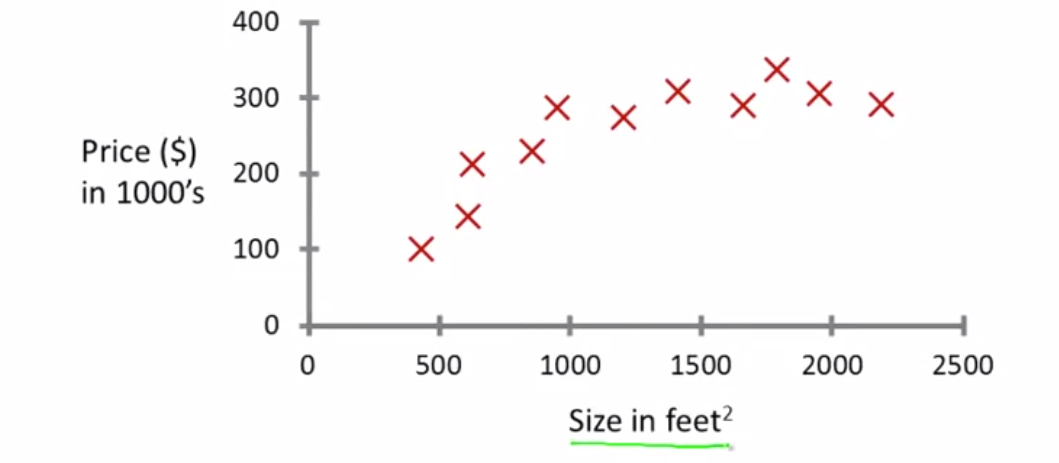
\includegraphics[width=0.7\linewidth]{screenshot001}
			\caption{Price vs. Size in Feet}
			\label{fig:screenshot001}
		\end{figure}
		\\\\\paragraph*{An Idea:} Provided we can plot a straight line through the data, we could use that to get a Y-axis value given some value on the X-axis
		\paragraph*{Perhaps a Better Idea:} Rather than a straight line what if we included a quadratic function
		\\\centerline{How do we decide which to use?}
		\\\\This is an example of a \emph{Regression Problem with Continuous Output}
		
		\subsubsection*{Example 2: Malignant Tumors}
		Given data about the size of a tumor can we predict whether it will be benign or malignant 
		\begin{figure}[h!]
			\centering
			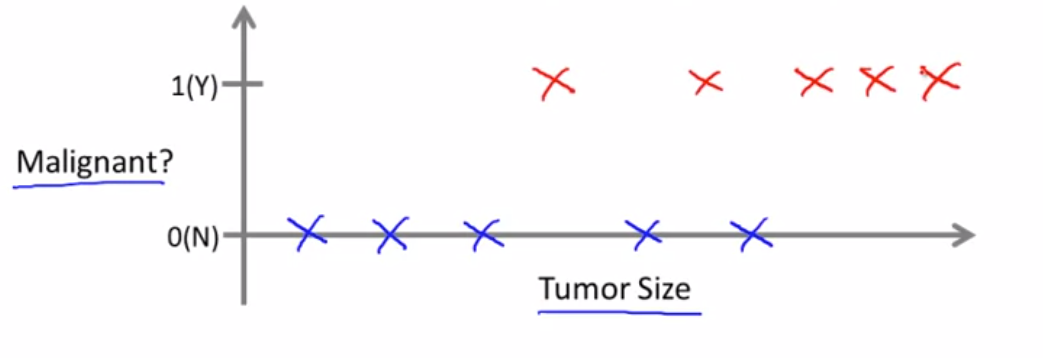
\includegraphics[width=0.7\linewidth]{screenshot002}
			\caption{Tumor Size vs. Malignant or Benign}
			\label{fig:screenshot002}
		\end{figure}
		This is an example of a \emph{Classification Problem}
		
		\paragraph*{Features} In above examples, the features Size in Feet$^{2}$ and Tumor Size were used as Inputs to the Machine Learning Algorithm. Mature Machine Learning approaches use many, many features. For example, in the Malignant Tumors exercise: Clump Thickness, Uniformity of Cell Size, and Uniformity of Cell Shape were all considered.
		
		\paragraph*{Support Vector Machine} A method to support including infinite amounts of features in a model. To discuss in detail later.
		
		
		
	\subsection*{\centerline{Unsupervised Learning}}
	\textsl{\centerline{Given data with no classification or labels, what do we do with it? How do we find structure?}}
	\paragraph*{Formal Definition} 
	
	\paragraph*{Clustering Algorithm} Group data points with no prior knowledge of relationship. Real world example: Google News finding new "stories"
	
	\begin{figure}[h!]
		\centering
		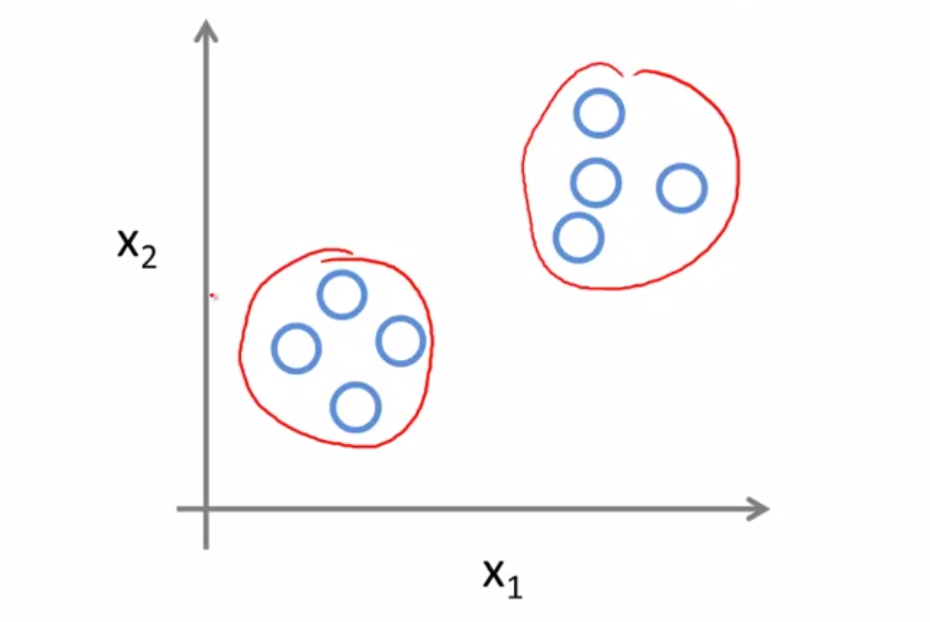
\includegraphics[width=0.7\linewidth]{screenshot003}
		\caption{Similar to the Malignant Tumor example, but here we cluster data points on our own with no guidance}
		\label{fig:screenshot003}
	\end{figure}

	
	
	
	

\section{Linear Regression with One Variable}

	\subsection*{\centerline{Model and Cost Function}}
	
		\subsubsection*{Model Representation}
		
		\subsubsection*{Cost Function}
	
	\subsection*{\centerline{Parameter Learning}}
		
		\subsubsection*{Gradient Descent}
		
		\subsubsection*{Gradient Descent in Linear Regression}

\section{Linear Algebra Review}

	\subsection*{\centerline{Matrices and Vectors}}
	
	\subsection*{\centerline{Addition and Scalar Multiplication}}
	
	\subsection*{\centerline{Matrix-Vector Multiplication}}
	
	\subsection*{\centerline{Matrix-Matrix Multiplication}}
	
	\subsection*{\centerline{Inverse and Transpose}}

\end{document}